\subsection{Cooperation Tactics and Tools}
The group work was coordinated primarily by using tools for planning, version control and communication. We generally applied a loose version of scrum to manage the project and become familiar with the SCRUM methodology. In practice we tried to keep each other updated every time we met (partial stand up) and would try to give each other an overview of three things accordingly; what did we do last, what are we planning to do today and finally whether anything is blocking this purpose. If anything was blocking a team member from continuing his work, the SCRUM facilitator would try to find the required help to solve this. 
We also established official meeting hours and contact periods to separate study related activities from social life. This was done to cope with the otherwise stressful environment that team members felt due to the heavy work load in this semester. Communication tools such as Facebook and Messenger were used to keep in contact and inform the group about practical information. Finally, the collaboration tool "Trello"  was used to keep track of everything. Note that all members are assumed to stay updated about changes on both Facebook, Git and Trello. 
\\
\textbf{Trello} is a collaboration tool we use to organize the project into so called "boards". In one glance, Trello tells you what's being worked on, who's working on what, and where something is in a process. The board represent a combination of the different phases used in SCRUM and the Waterfall Model. We have a Backlog board that corresponds to the Product backlog containing all possible features and requirements in the system. Secondly, the Sprint board contains a backlog with a work that must be addressed during the next sprint (usually one for each week). When team members finish a task it is tested and reviewed by another member in the other boards and finally put in the Done board. 

\begin{figure}[H]
	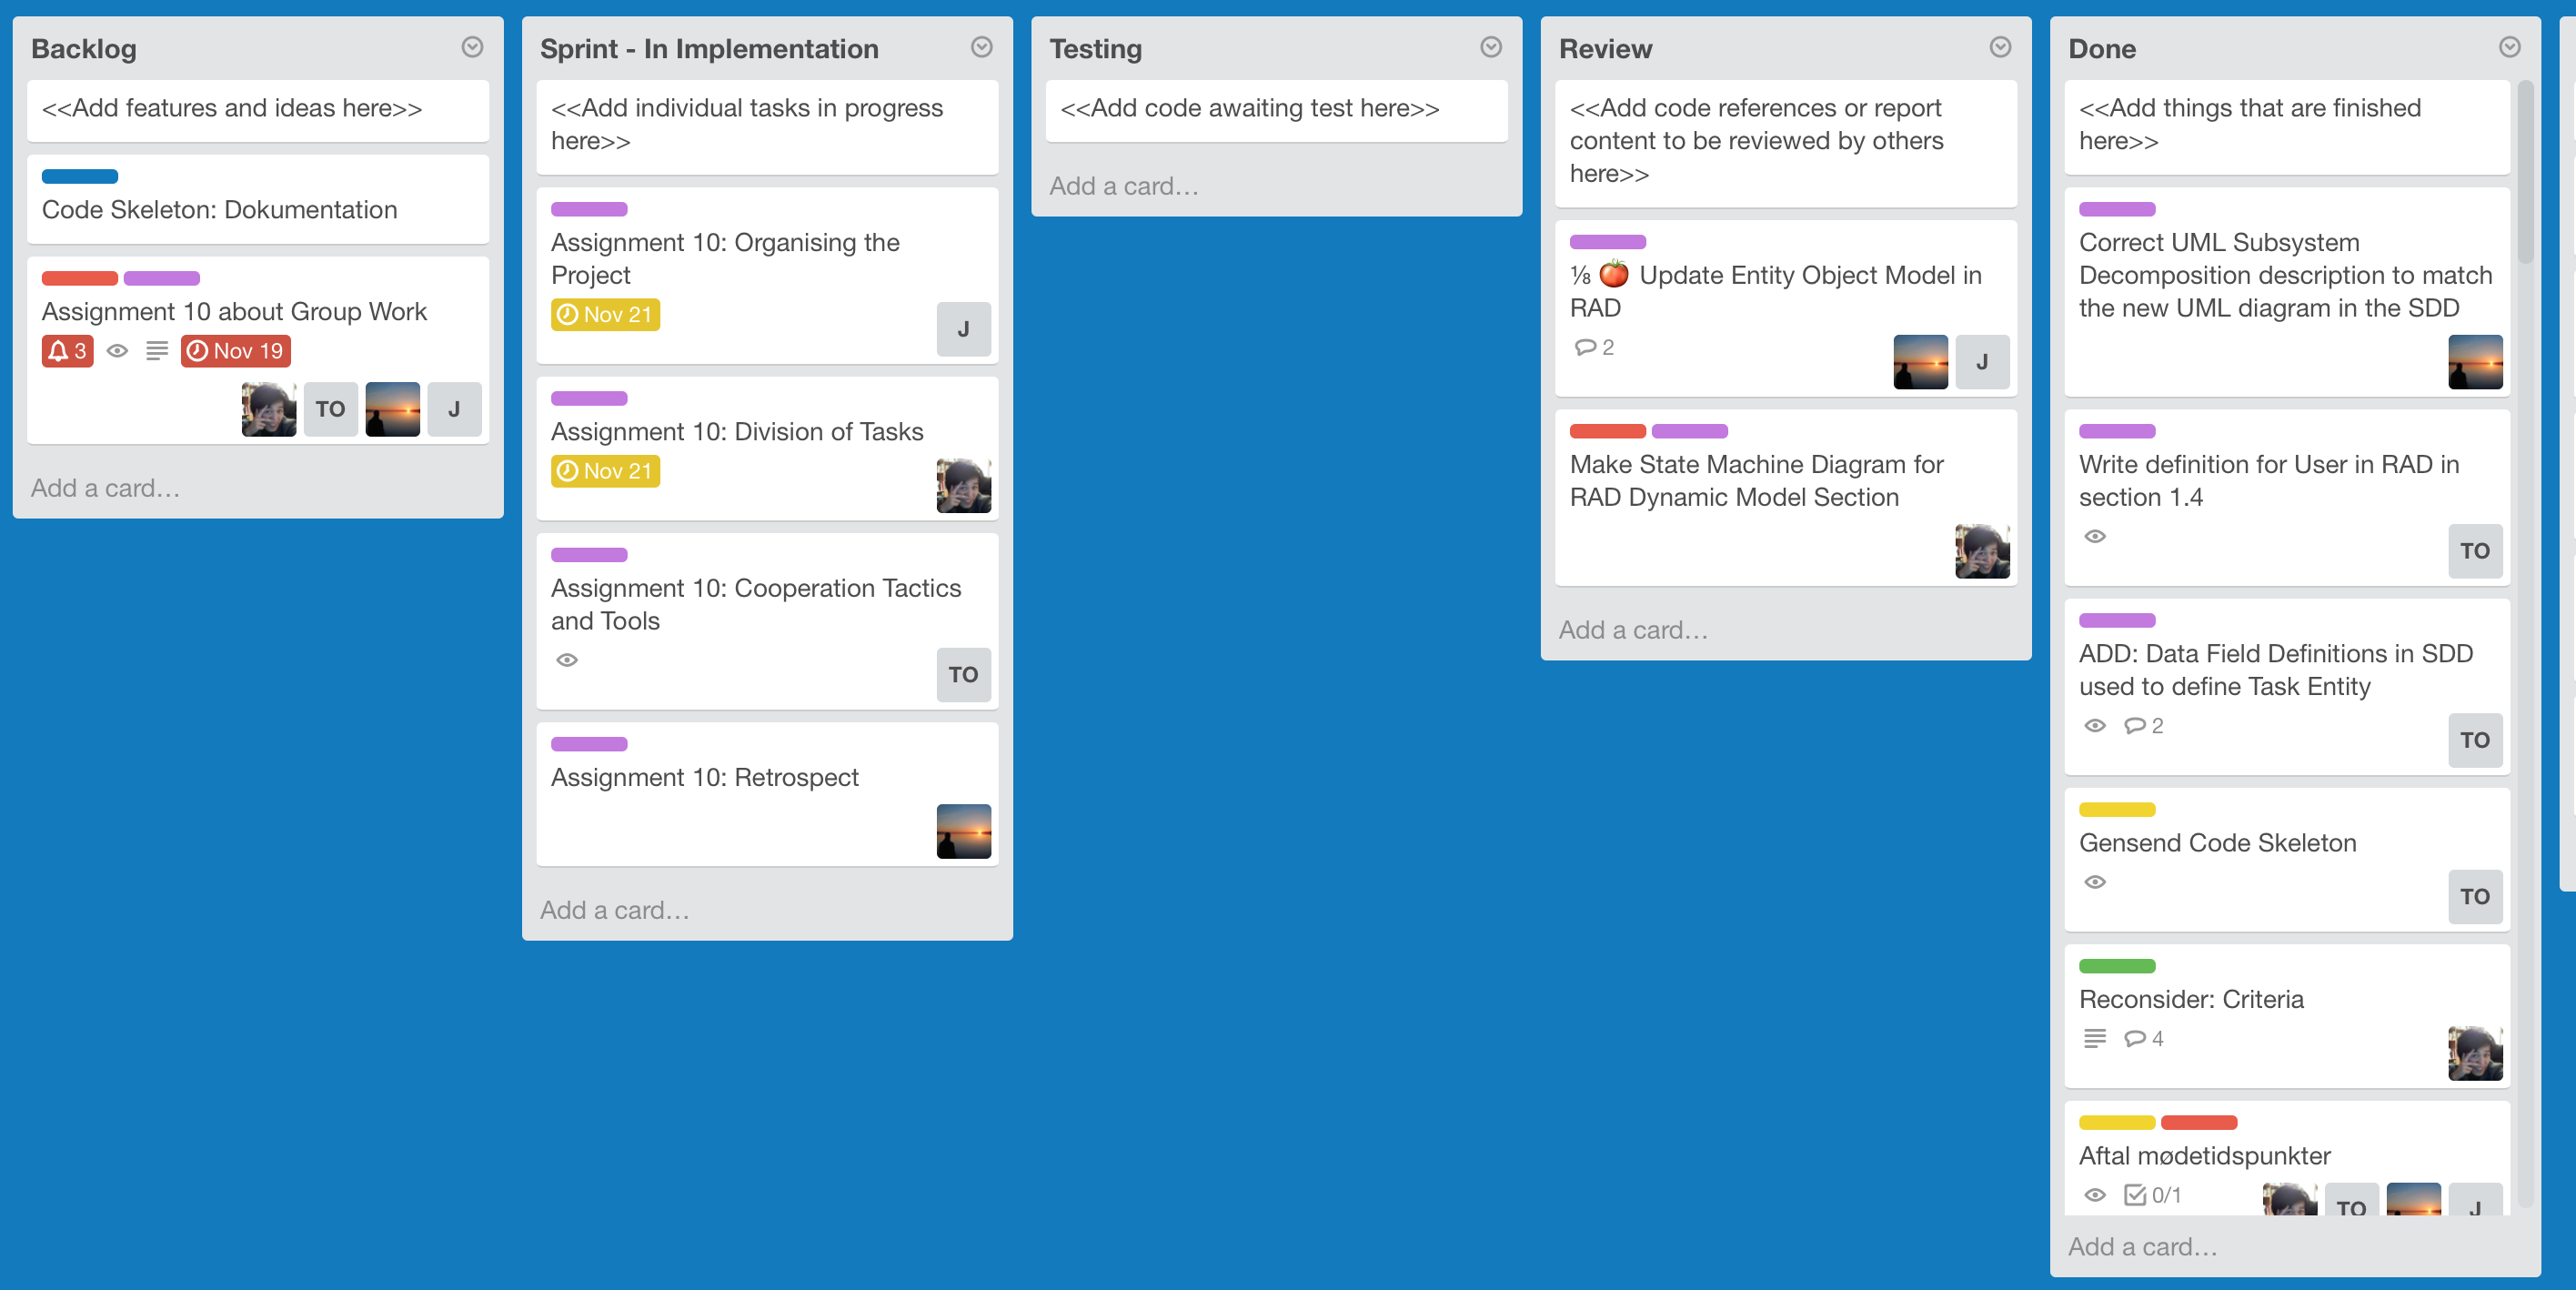
\includegraphics[width=\linewidth]{trello}
	\caption{Trello Board}
	\label{fig:trello}
\end{figure}
